\documentclass[aspectratio=1610, xcolor=table]{beamer}


\usepackage{listings}
\usepackage{alltt}

\usepackage{tikz}
\usepackage{tikz-qtree}
\usepackage{multirow}
\usepackage{subfig}
\def\addsquare#1{\tikz\node[draw]{#1};}
\def\addcircle#1{\tikz\node[draw,circle]{#1};}



\usepackage{xcolor}
\definecolor{pgreen}{rgb}{0,0.5,0}

\usetheme{Antibes}

\lstset{
    language=Java,
    showstringspaces=false,
    columns=flexible,
    basicstyle={\small\ttfamily},
    numbers=none,
    numberstyle=\tiny\color{gray},
    keywordstyle=\color{blue},
    commentstyle=\color{pgreen},
    stringstyle=\color{pgreen},
    breaklines=true,
    breakatwhitespace=true,
    tabsize=3,
    escapeinside={(*}{*)},
    aboveskip=-1em,
    belowskip=-1em,
}

%Information to be included in the title page:
\title{Incremental clone detection for IDEs using dynamic suffix arrays}
\author{Jakob Konrad Hansen}
\institute{University of Oslo}
\date{2023}



\begin{document}

\frame{\titlepage}

\begin{frame}
    \frametitle{Outline}
    \tableofcontents
\end{frame}

\section{Motivation and contribution}

\begin{frame}
\frametitle{Motivation}
\begin{itemize}
    \item Duplicated code is generally considered harmful to software quality
    \item Software often contains $10-15\%$ duplicated code
    \item Code clone detection, analysis and management is therefore important
    \item Incremental clone detection algorithms have not been thoroughly researched
    \item Incremental algorithms are useful in use-cases such as in IDEs
\end{itemize}
\end{frame}

\begin{frame}
\frametitle{Our contribution}
\begin{itemize}
    \item CCDetect-LSP: An incremental clone detection tool for IDEs
    \item Uses a novel application of dynamic extended suffix arrays for clone detection
    \item Language- and IDE agnostic via Tree-sitter and LSP
\end{itemize}
\end{frame}

\section{Background}

\subsection{Code clone theory}

\begin{frame}
    \frametitle{Code clones}

    \begin{definition}[Code snippet]
        A code snippet is a piece of contiguous source code in a larger software system.
    \end{definition}

    \begin{definition}[Code clone]
        A code clone is a code snippet which is equal or similar to another code snippet. The two
        code snippets are both code clones, and together they form a clone pair. 
    \end{definition}
\end{frame}

\begin{frame}[fragile]
	\frametitle{Clone types: type-1 and type-2}
    \begin{figure}[t]
		\begin{center}
			\begin{tabular}{c | c}
				\begin{lstlisting}
for (int i = 0; i < 10;   i++) {
    print(i);
}
\end{lstlisting} &
				\begin{lstlisting}
for (int i = 0; i < 10; i++) {
    // A comment

    print(i);
}
            \end{lstlisting}
			\end{tabular}
		\end{center}
        \caption{Type-1 clone pair}
    \end{figure}
    \begin{figure}[t]
        	\begin{center}
        \begin{tabular}{p{6cm} | p{6cm}}
\begin{lstlisting}
for (int i = 0; i < 10; i++) {
    print(i);
}
\end{lstlisting} & \begin{lstlisting}
for (int (*\textbf j*) = (*\textbf 5*); (*\textbf j*) < (*\textbf{20}*); (*\textbf j++*)) {
    print((*\textbf j*));
}
\end{lstlisting}
		\end{tabular}
	\end{center}

        \caption{Type-2 clone pair}
    \end{figure}

\end{frame}

\subsection{Preliminary algorithms and data structures}
\begin{frame}{Parsing and incremental parsing}
    \begin{figure}
        \begin{center}
            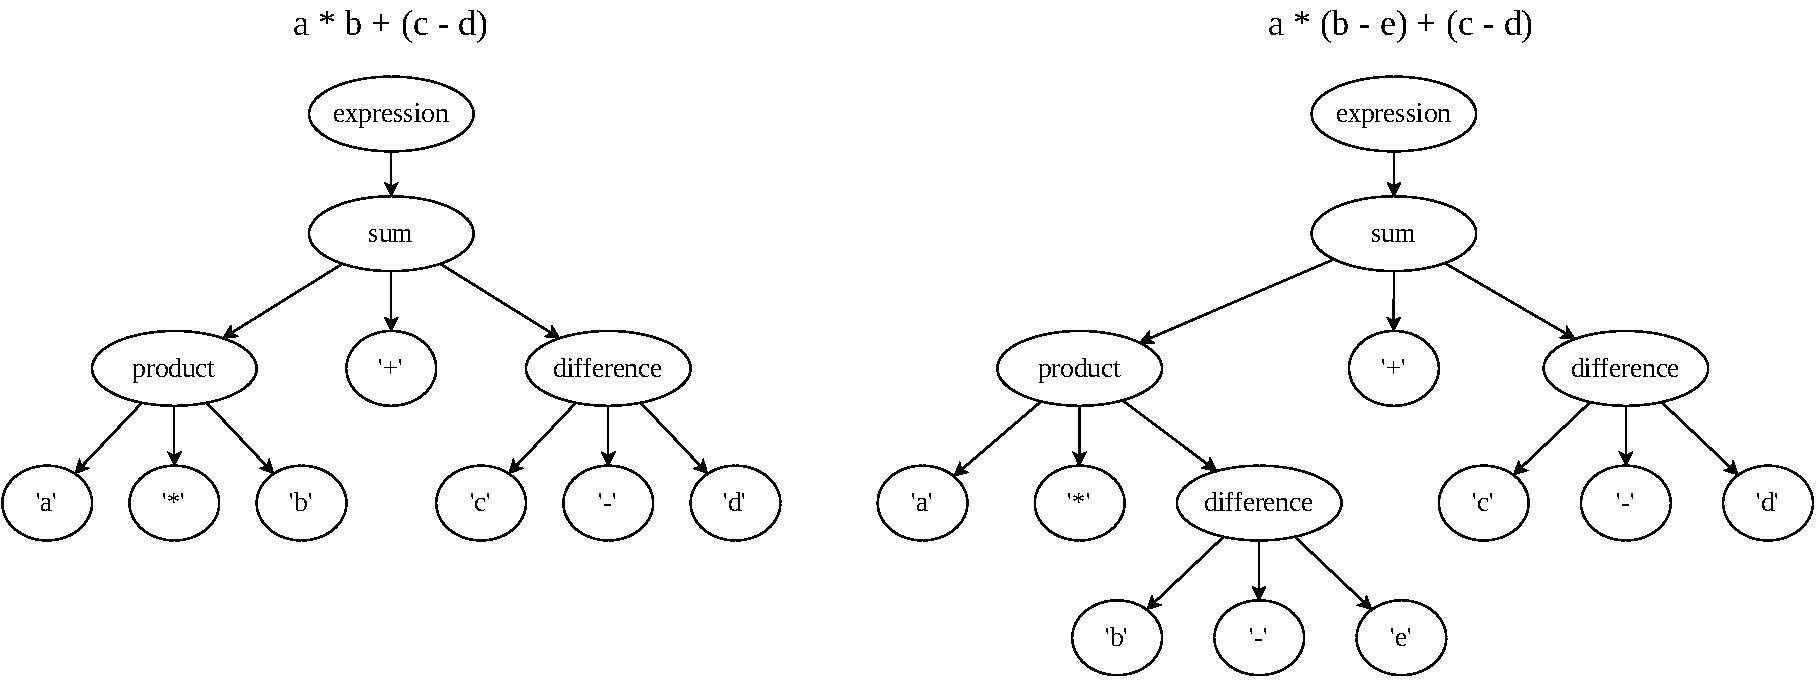
\includegraphics[width=0.95\textwidth]{figures/incrementalparsing1.drawio.pdf}
        \end{center}
    \end{figure}
\end{frame}

\begin{frame}{Parsing and incremental parsing}
    \begin{figure}
        \begin{center}
            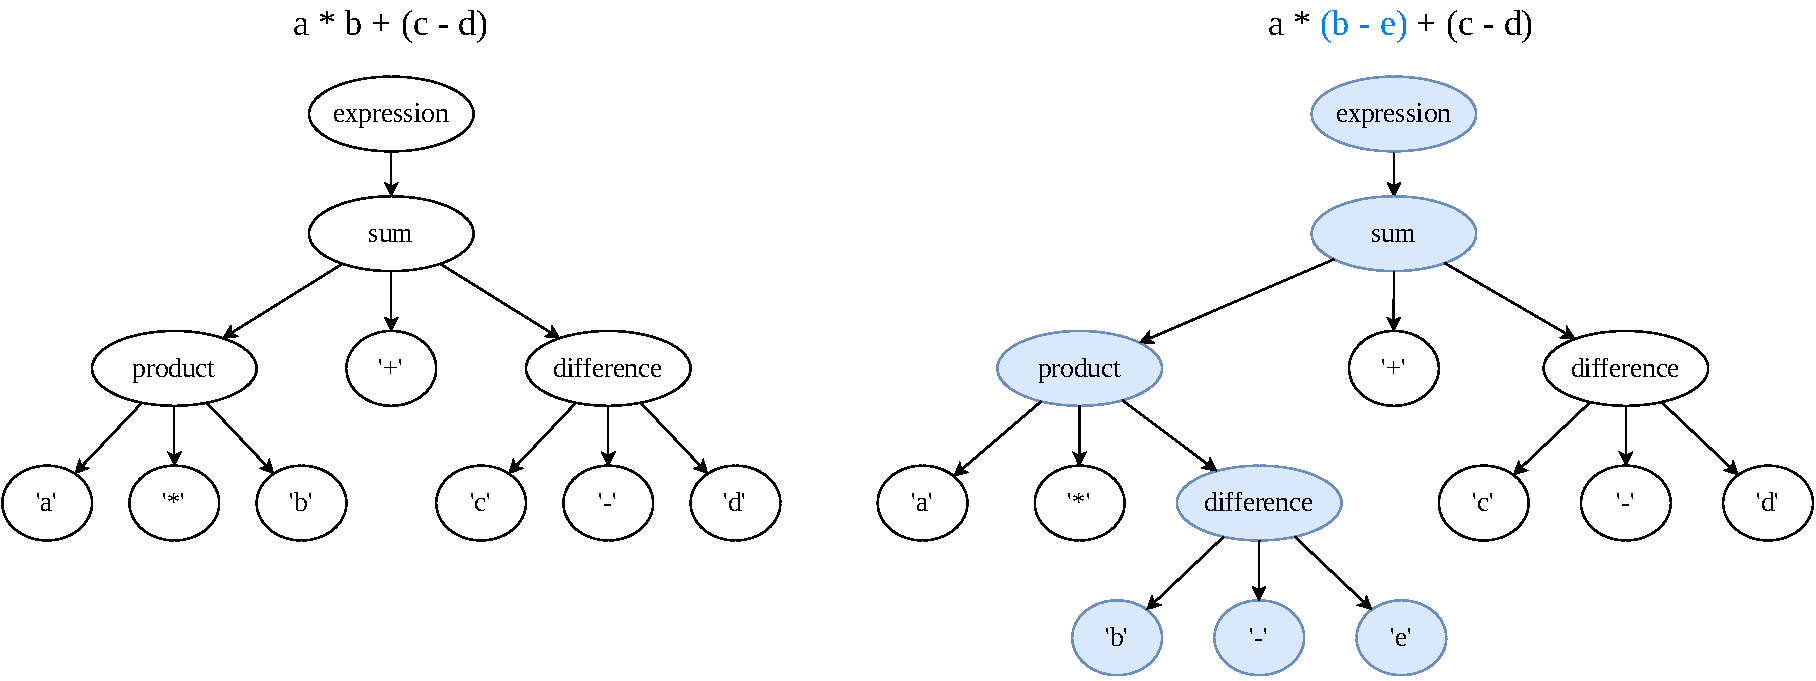
\includegraphics[width=0.95\textwidth]{figures/incrementalparsing2.drawio.pdf}
        \end{center}
    \end{figure}
\end{frame}

\begin{frame}{Suffix array}
	\begin{table}
		\begin{center}
			\subfloat[Suffixes]{
				\begin{tabular}{c | l }
					Index & Suffix   \\
					\hline
					0     & BANANA\$ \\
					1     & ANANA\$  \\
					2     & NANA\$   \\
					3     & ANA\$    \\
					4     & NA\$     \\
					5     & A\$      \\
					6     & \$       \\
				\end{tabular}}
			\hspace{1cm}
			\subfloat[Sorted suffixes]{\begin{tabular}{c | l}
					Index & Suffix   \\
					\hline
					6     & \$       \\
					5     & A\$      \\
					3     & ANA\$    \\
					1     & ANANA\$  \\
					0     & BANANA\$ \\
					4     & NA\$     \\
					2     & NANA\$   \\
				\end{tabular}}
			\hspace{1cm}
			\subfloat[SA, ISA and LCP]{\begin{tabular}{c | c | c | c}
					Index & SA & ISA & LCP \\
					\hline
					0     & 6  & 4   & 0   \\
					1     & 5  & 3   & 0   \\
					2     & 3  & 6   & 1   \\
					3     & 1  & 2   & 3   \\
					4     & 0  & 5   & 0   \\
					5     & 4  & 1   & 0   \\
					6     & 2  & 0   & 2   \\
				\end{tabular}}
		\end{center}
	\end{table}

\end{frame}
    
\begin{frame}{Burrows-Wheeler transform}
    \begin{table}
	\begin{center}
        \subfloat[Cyclic shifts]{
		\begin{tabular}{c | l }
			Index & CS   \\
			\hline
			0     & BANANA\$ \\
			1     & ANANA\$B \\
			2     & NANA\$BA \\
			3     & ANA\$BAN \\
			4     & NA\$BANA \\
			5     & A\$BANAN \\
			6     & \$BANANA \\
    \end{tabular}}
		\hspace{0.25cm}
        \subfloat[Sorted cyclic shifts and BWT]{\begin{tabular}{c | l}
			Index & CS   \\
			\hline
            6     & \$BANAN\textbf{A} \\
            5     & A\$BANA\textbf{N} \\
			3     & ANA\$BA\textbf{N} \\
			1     & ANANA\$\textbf{B} \\
			0     & BANANA\textbf{\$} \\
			4     & NA\$BAN\textbf{A} \\
			2     & NANA\$B\textbf{A} \\
    \end{tabular}}
		\hspace{0.25cm}
        \subfloat[LF function]{\begin{tabular}{c | l}
			L & F   \\
			\hline
            0     & $Rank_A(0) + C[A] = 0 + 1 = 1$\\
            1     & $Rank_N(1) + C[N] = 0 + 5 = 5$ \\
			2     & $Rank_N(2) + C[N] = 1 + 5 = 6$ \\
			3     & $Rank_B(3) + C[B] = 0 + 4 = 4$ \\
            4     & $Rank_{\$}(4) + C[\$] = 0 + 0 = 0$ \\
			5     & $Rank_A(5) + C[A] = 1 + 1 = 2$ \\
			6     & $Rank_A(6) + C[A] = 2 + 1 = 3$ \\
    \end{tabular}}
    \caption{S = BANANA\$, BWT = ANNB\$AA}
    \label{table:bwt}
	\end{center}
\end{table}
\end{frame}

\section{Implementation}

\subsection{Features}

\begin{frame}{CCDetect-LSP features}
    \begin{columns}
        \column{0.55\linewidth}{
	\begin{itemize}
		\item CCDetect-LSP is implemented as an LSP server
            \begin{itemize}
                \item List clones
                \item Display clones inline with code
                \item Jump between matching clones
                \item Incremental updates on each edit
            \end{itemize}
	\end{itemize}
        }
        \column{0.45\linewidth}{
            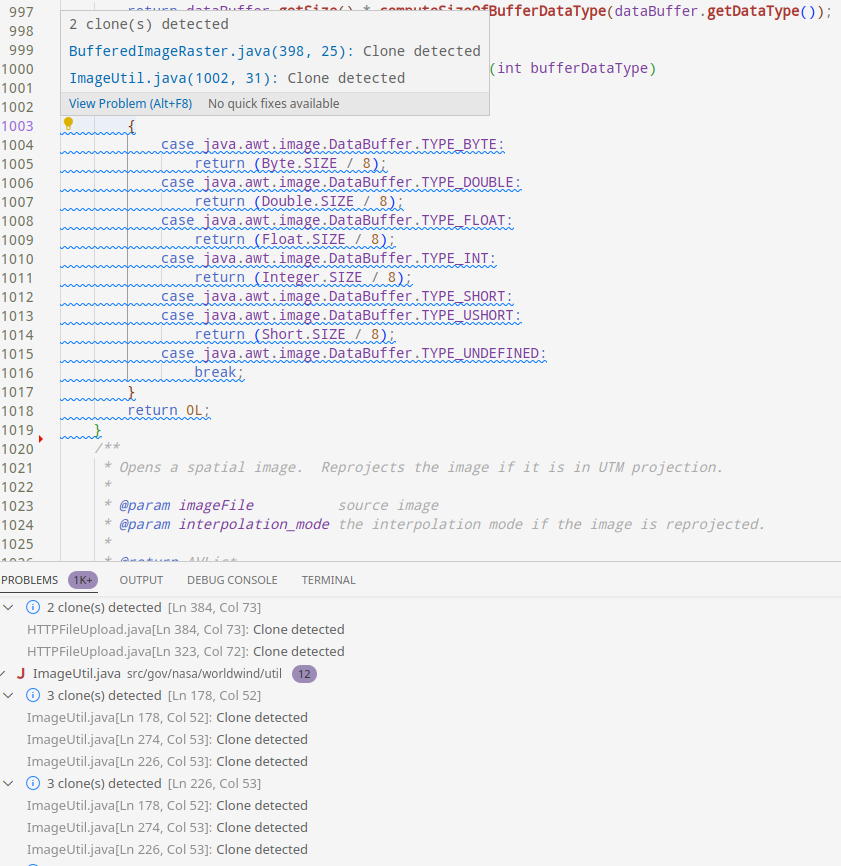
\includegraphics[width=0.95\textwidth]{figures/vscodecodeclone.png}
        }
    \end{columns}
\end{frame}

\subsection{Initial clone detection}

\begin{frame}{Implementation: Initial clone detection}
    \begin{itemize}
        \item Algorithm which initially detects type-1 and optionally type-2 clones
        \item Pipeline of 5 phases, returns a list of clones
        \item Uses an extended suffix array for match detection
    \end{itemize}
\end{frame}

\begin{frame}{Detection algorithm overview}
    \begin{figure}
        \begin{center}
            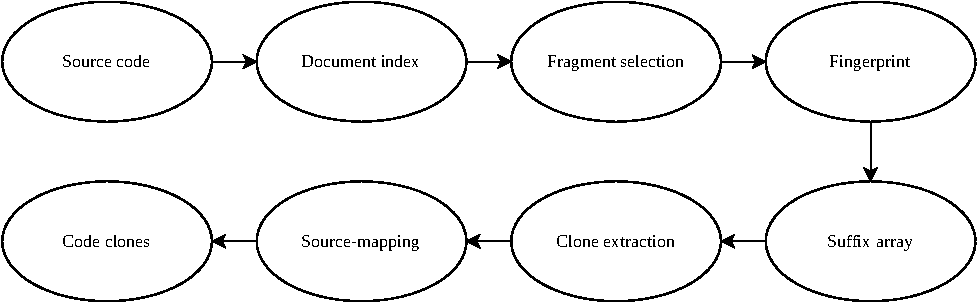
\includegraphics[width=0.95\textwidth]{figures/phases_all.drawio.pdf}
        \end{center}
        \caption{Overview of detection algorithm phases}
    \end{figure}
\end{frame}

\begin{frame}[fragile]{Phase 1: Fragment selection}
    \begin{itemize}
        \item Parse files using Tree-sitter
        \item Use a configurable Tree-sitter query to ``capture'' nodes
        \item Extract and store the tokens of captured nodes
    \end{itemize}
    \vspace{1cm}
    \begin{center}
        \verb|(method_declaration) @method (constructor_declaration) @constructor|
    \end{center}
\end{frame}

	\newsavebox{\firstlisting}
	\begin{lrbox}{\firstlisting}
        \begin{lstlisting}
            public class Math() {
                public int multiplyByTwo(int param) {
                    return param * 2;
                }

                public int addTwo(int param) {
                    return param + 2;
                }
            }
        \end{lstlisting}
	\end{lrbox}
\begin{frame}[fragile]{Phase 2: Fingerprinting}
    \begin{itemize}
        \item Consistently hash each token value with an increasing integer counter
        \item For type-2 detection, hash the token type instead
    \end{itemize}
	\begin{figure}
		\begin{center}
            \scalebox{.75}{\usebox{\firstlisting}}
                \hspace{.5cm}
                \scalebox{.7}{\begin{tabular}{l | l}
					Token         & Fingerprint \\
					\hline
					public        & 2           \\
					int           & 3           \\
					multiplyByTwo & 4           \\
					(             & 5           \\
					param         & 6           \\
					)             & 7           \\
					\{            & 8           \\
					return        & 9           \\
					*             & 10          \\
					2             & 11          \\
					;             & 12          \\
					\}            & 13          \\
					addTwo        & 14          \\
					+             & 15          \\
            \end{tabular}}
            \vspace{.5cm}

            [ 2, 3, 4, 5, 3, 6, 7, 8, 9, 6, 10, 11, \underline{1}, 2, 3, 14, 5, 3, 6, 7,
                    8, 9, 6, 15, 11, \underline{1}, \underline{0} ]
		\end{center}
		\label{fig:fingerprint}
	\end{figure}
\end{frame}

\begin{frame}[fragile]{Phase 3: Suffix array construction}
    \begin{itemize}
        \item Concatenate the fingerprints of each document in the index
        \item Construct SA, ISA and LCP array of the full fingerprint
        \item Uses ``Induced sorting variable-length LMS-substrings'' (SA-IS) algorithm
        \item LCP algorithm slightly modified
    \end{itemize}

\end{frame}

\begin{frame}{Phase 4: Clone extraction}
    \begin{columns}
        \column{0.5\textwidth}{
            \begin{itemize}
                \item Use SA, ISA and LCP to find clone positions
                \item Linear scan through the fingerprint
                \item Skip contained clones
            \end{itemize}
        }
        \column{0.5\textwidth}{
            \scalebox{.75}{\usebox{\firstlisting}}
        }
    \end{columns}
    \begin{center}
        \begin{table}
        
            \setlength{\tabcolsep}{2pt}
        \begin{tabular}{c|ccccccccccccccccccccccccccc}
            F & 2 & 3 & 4 & {\color{blue}5} & {\color{blue}3} & {\color{blue}6}
              &{\color{blue} 7} & {\color{blue}8} & {\color{blue}9} & {\color{blue}6} & 10 & 11 & 1 & 2 & 3 & 14 &
            {\color{blue}5} & {\color{blue}3} & {\color{blue}6} & {\color{blue}7} &
            {\color{blue}8} & {\color{blue}9} & 6 & 15 & 11 & 1 & 0 \\
        SA & 26 & 25 & 12 & 0 & 13 & 1 & 4 & 17 & 14 & 2 & {\color{blue}3} &
        {\color{blue}16} & 5 & 18 & 9 & 22 & 6 & 19 & 7 & 20 & 8 & 21 & 10 & 24 & 11 & 15 & 23 \\
        ISA & 3 & 5 & 9 & 10 & 6 & 12 & 16 & 18 & 20 & 14 & 22 & 24 & 2 & 4 & 8 & 25 & {\color{blue}11} & 7 & 13 & 17 & 19 & 21 & 15 & 26 & 23 & 1 & 0 \\
        LCP & 0 &  0 &  0 &  0 &  2 &  0 &  1 &  6 &  1 &  0 &  0 &  {\color{blue} 7} &  0 &  5 &  1 &  1 &  0 &  4 &  0 &  3 &  0 &  2 &  0 &  0 &  1 &  0 &  0
        \end{tabular}
        \end{table}
    \end{center}
\end{frame}

\begin{frame}{Phase 5: Source-mapping}
    \begin{itemize}
        \item Map the positions of clones back to the original source-code
        \item Find the correct file and position of an index in the fingerprint
        \item Binary-search speeds this process up
    \end{itemize}
\end{frame}


\subsection{Incremental clone detection}
\begin{frame}{Implementation: Incremental clone detection}
    \begin{itemize}
        \item Convert the algorithm to an incremental one
        \item Input is now the file(s) which has changed and the range(s)
        \item Dynamic suffix array with edit operations as input
    \end{itemize}
\end{frame}

\begin{frame}{Phase 1 and 2: Fragment selection and fingerprinting}
    \begin{itemize}
        \item Mainly reuse results from previous computation, except for changed file
        \item Fragment selection
    \begin{itemize}
        \item Store the AST of the opened files
        \item Incrementally parse the changed file with Tree-sitter
    \end{itemize}
\item Fingerprinting
    \begin{itemize}
        \item Each document stores its fingerprint
        \item Only need to fingerprint (and fragment select) changed files
    \end{itemize}
    \end{itemize}
\end{frame}


\begin{frame}[fragile]{Phase 2.5: Edit operations}
	\begin{columns}
		\column{0.45\linewidth}{
			\begin{itemize}
				\item Input to phase 3: Edit operations
				\item How to determine edit operations?
				\item Edit distance algorithm!
				\item ``Batched'' operations preferred
			\end{itemize}
		}
		\column{0.55\linewidth}{
			\begin{table}
				\begin{center}
					\begin{tabular}[c]{c|c|c|c|c|c|c|c|c|c|}
						  &                      & D                    & E                    & M                    & O                    & C                    & R                    & A                    & T                    \\\hline
						  & \cellcolor{blue!25}0 & 1                    & 2                    & 3                    & 4                    & 5                    & 6                    & 7                    & 8                    \\\hline
						R & 1                    & \cellcolor{blue!25}1 & 2                    & 3                    & 4                    & 5                    & 5                    & 6                    & 7                    \\\hline
						E & 2                    & 2                    & \cellcolor{blue!25}1 & 2                    & 3                    & 4                    & 5                    & 6                    & 7                    \\\hline
						P & 3                    & 3                    & \cellcolor{blue!25}2 & 2                    & 3                    & 4                    & 5                    & 6                    & 7                    \\\hline
						U & 4                    & 4                    & \cellcolor{blue!25}3 & 3                    & 3                    & 4                    & 5                    & 6                    & 7                    \\\hline
						B & 5                    & 5                    & 4                    & \cellcolor{blue!25}4 & 4                    & 4                    & 5                    & 6                    & 7                    \\\hline
						L & 6                    & 6                    & 5                    & 5                    & \cellcolor{blue!25}5 & 5                    & 5                    & 6                    & 7                    \\\hline
						I & 7                    & 7                    & 6                    & 6                    & 6                    & \cellcolor{blue!25}6 & 6                    & 6                    & 7                    \\\hline
						C & 8                    & 8                    & 7                    & 7                    & 7                    & 6                    & \cellcolor{blue!25}7 & 7                    & 7                    \\\hline
						A & 9                    & 9                    & 8                    & 8                    & 8                    & 7                    & 7                    & \cellcolor{blue!25}7 & 8                    \\\hline
						N & 10                   & 10                   & 9                    & 9                    & 9                    & 8                    & 8                    & 8                    & \cellcolor{blue!25}8 \\\hline

						\hline
					\end{tabular}
				\end{center}
				\caption{REPUBLICAN $\rightarrow$ DEMOCRAT}
				\label{tab:wagnerfischermatrix}
			\end{table}
		}
	\end{columns}
\end{frame}

\begin{frame}[fragile]{Optimize edit distance}
\begin{columns}
	\column{0.4\linewidth}{
		\begin{itemize}
			\item Standard algorithm memory usage is too high
			\item Need to optimize
			      \begin{itemize}
				      \item Compare new/old fingerprint of changed document only
				      \item Remove trivial part at each end of matrix
				      \item Hirschberg's algorithm
			      \end{itemize}
		\end{itemize}
	}
	\column{0.6\linewidth}{
        \begin{table}
			\begin{center}
                \scalebox{.9}{\begin{tabular}[c]{c|c|c|c|c|c|c|c|c|c|c|}
					  &                      & F                     & I                     & N                     & I                     & S                     & H                     & I                    & N                    & G                    \\\hline
					  & \cellcolor{blue!25}0 & 1                     & 2                     & 3                     & 4                     & 5                     & 6                     & 7                    & 8                    & 9                    \\\hline
					F & 1                    & \cellcolor{blue!25}0  & \cellcolor{green!25}1 & \cellcolor{green!25}2 & \cellcolor{green!25}3 & \cellcolor{green!25}4 & \cellcolor{green!25}5 & 6                    & 7                    & 8                    \\\hline
					A & 2                    & \cellcolor{green!25}1 & \cellcolor{blue!25}1  & \cellcolor{green!25}2 & \cellcolor{green!25}3 & \cellcolor{green!25}4 & \cellcolor{green!25}5 & 6                    & 7                    & 8                    \\\hline
					S & 3                    & \cellcolor{green!25}2 & \cellcolor{green!25}2 & \cellcolor{blue!25}2  & \cellcolor{green!25}3 & \cellcolor{green!25}3 & \cellcolor{green!25}4 & 5                    & 6                    & 7                    \\\hline
					C & 4                    & \cellcolor{green!25}3 & \cellcolor{green!25}3 & \cellcolor{blue!25}3  & \cellcolor{green!25}3 & \cellcolor{green!25}4 & \cellcolor{green!25}4 & 5                    & 6                    & 7                    \\\hline
					I & 5                    & \cellcolor{green!25}4 & \cellcolor{green!25}3 & \cellcolor{green!25}4 & \cellcolor{blue!25}3  & \cellcolor{green!25}4 & \cellcolor{green!25}5 & 4                    & 5                    & 6                    \\\hline
					N & 6                    & \cellcolor{green!25}5 & \cellcolor{green!25}4 & \cellcolor{green!25}3 & \cellcolor{green!25}4 & \cellcolor{blue!25}4  & \cellcolor{green!25}5 & 5                    & 4                    & 5                    \\\hline
					A & 7                    & \cellcolor{green!25}6 & \cellcolor{green!25}5 & \cellcolor{green!25}4 & \cellcolor{green!25}4 & \cellcolor{green!25}5 & \cellcolor{blue!25}5  & 6                    & 5                    & 5                    \\\hline
					T & 8                    & \cellcolor{green!25}7 & \cellcolor{green!25}6 & \cellcolor{green!25}5 & \cellcolor{green!25}5 & \cellcolor{green!25}5 & \cellcolor{blue!25}6  & 6                    & 6                    & 6                    \\\hline
					I & 9                    & 8                     & 7                     & 6                     & 5                     & 6                     & 6                     & \cellcolor{blue!25}6 & 7                    & 7                    \\\hline
					N & 10                   & 9                     & 8                     & 7                     & 6                     & 6                     & 7                     & 7                    & \cellcolor{blue!25}6 & 7                    \\\hline
					G & 11                   & 10                    & 9
                      & 8                     & 7                     & 7
                      & 7                     & 8                    & 7
                      & \cellcolor{blue!25}6 \\\hline\end{tabular}} \end{center}
                      \caption{FASCINATING $\rightarrow$ FINISHING \\ ASCINAT $\rightarrow$
                      INISH}
			\label{tab:minimizededitmatrix}
    \end{table}

	}
\end{columns}
\end{frame}

\begin{frame}{Phase 3: Dynamic suffix array}
    \begin{itemize}
        \item Update suffix array based on edit operations
        \item ``Four-stage algorithm for updating a Burrows-Wheeler transform''
        \item Updates to the BWT correlates with updates to the SA and ISA
    \end{itemize}
\end{frame}

\begin{frame}[fragile]{Phase 3: Dynamic suffix array}
	\begin{table}
		\begin{center}
			\subfloat[Original BWT]{
				\begin{tabular}{c | l | l}
					Order & F  & L  \\
					\hline
					6     & \$ & A  \\
					5     & A  & N  \\
					3     & A  & N  \\
					1     & A  & B  \\
					0     & B  & \$ \\
					4     & N  & A  \\
					2     & N  & A  \\
				\end{tabular}
			}
			\hspace{0.5cm}
			\subfloat[After change and insert]{
				\begin{tabular}{c | l | l l}
					Order & F          & L                              \\
					\hline
					7     & \$         & A          &                   \\
					6     & A          & N          &                   \\
					4     & A          & N          &                   \\
					1     & A          & B          &                   \\
					0     & B          & \$         &                   \\
					2     & \textbf{B} & \textbf{A} & Inserted          \\
					5     & B          & A          &                   \\
					3     & \textbf{N} & \textbf{B} & $A \rightarrow B$ \\
				\end{tabular}
			}
			\hspace{0.5cm}
			\subfloat[After reordering]{
				\begin{tabular}{c | l | l l}
					Order & F          & L          &                                 \\
					\hline
					7     & \$         & A          &                                 \\
					6     & A          & N          &                                 \\
					1     & \textbf{A} & \textbf{B} & \multirow{2}{*}{$\updownarrow$} \\
					4     & \textbf{A} & \textbf{N} &                                 \\
					0     & B          & \$         &                                 \\
					2     & B          & A          &                                 \\
					5     & B          & A          &                                 \\
					3     & N          & B          &                                 \\
				\end{tabular}
			}
			\caption{Updating BWT dynamically for the string BANANA\$ $\rightarrow$ BABNANA\$}
			\label{table:bwtupdatestages}
		\end{center}
	\end{table}
\end{frame}

\begin{frame}[fragile]{Dynamic extended suffix array}
    \begin{itemize}
        \item Updating suffix array is slow $(O(n))$, new data structure needed
    \end{itemize}
	\begin{figure}[t]
		\begin{center}
			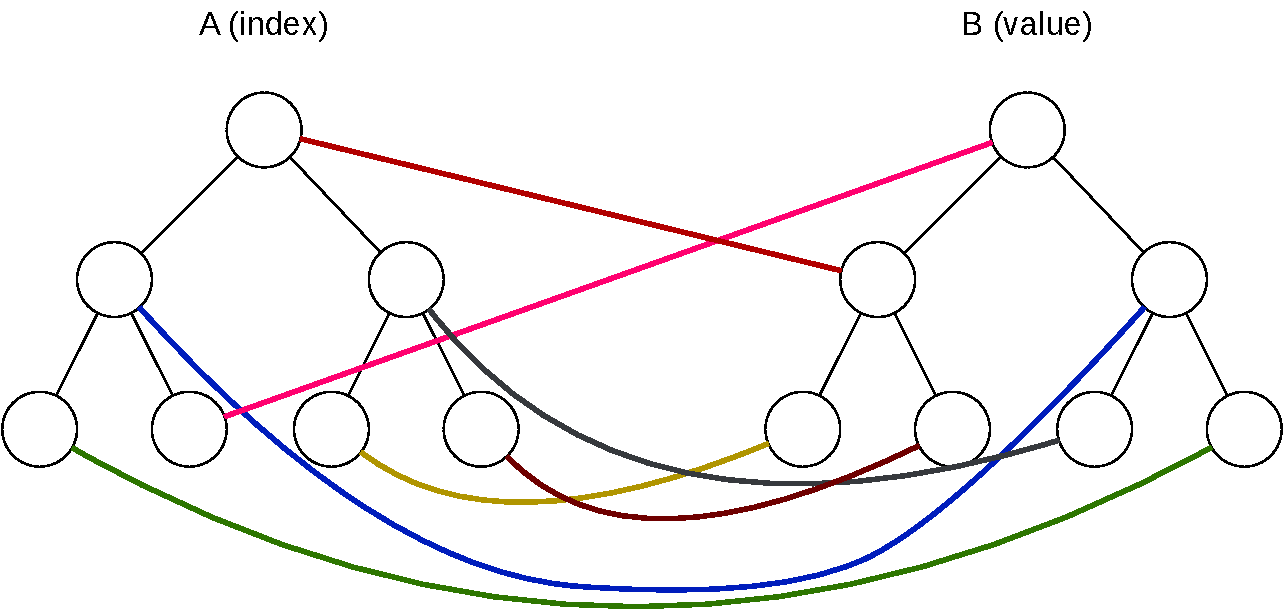
\includegraphics[width=0.9\textwidth]{figures/dynamicpermutation1.drawio.pdf}
		\end{center}
		\caption{Dynamic permutation for the permutation $[6,5,3,1,0,4,2]$.}
		\label{fig:dynamicpermutation}
	\end{figure}
\end{frame}

\begin{frame}[fragile]{Dynamic extended suffix array}
    \begin{itemize}
        \item Updating suffix array is slow $(O(n))$, new data structure needed
    \end{itemize}
	\begin{figure}[t]
		\begin{center}
			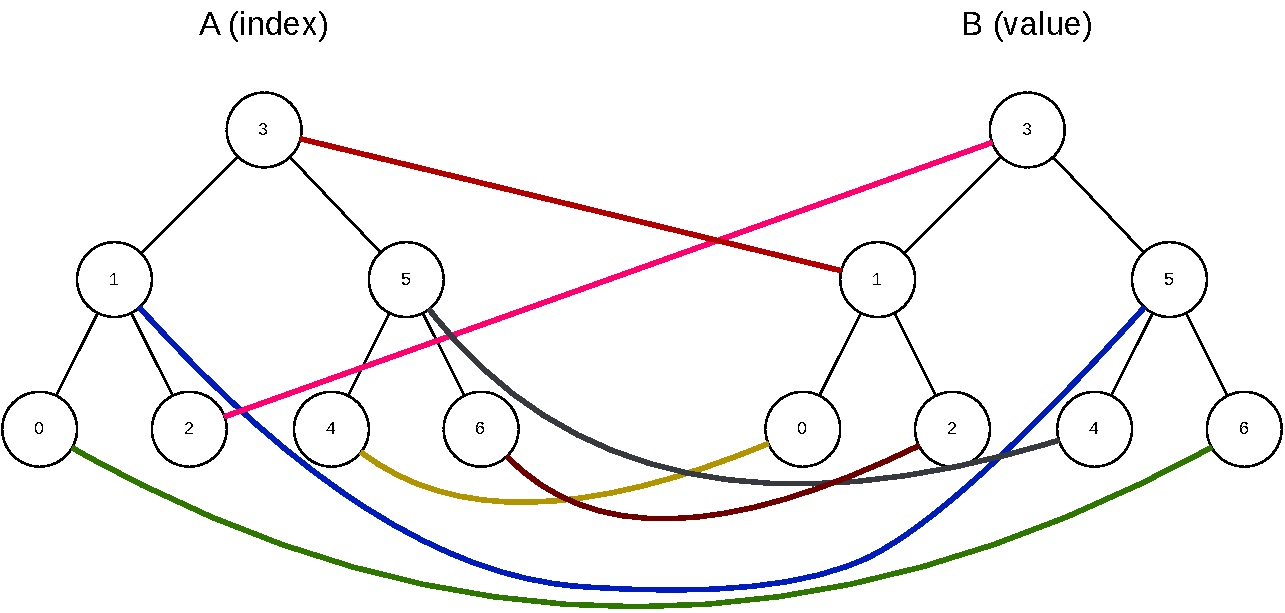
\includegraphics[width=0.9\textwidth]{figures/dynamicpermutation2.drawio.pdf}
		\end{center}
		\caption{Dynamic permutation for the permutation $[6,5,3,1,0,4,2]$.}
		\label{fig:dynamicpermutation}
	\end{figure}
\end{frame}

\begin{frame}[fragile]{Updating LCP values}
    \begin{itemize}
        \item SA updates correlate with LCP values which need to be updated
    \end{itemize}
    \begin{table}[t]
	\begin{center}
		\scalebox{1.5}{
			\begin{tabular}[c]{c|cccccccc}
				              &               &     & \multicolumn{2}{c}{$\leftrightarrow$}
				              &               & INS &                                       &                                           \\
				BWT           & A             & N   & B                                     & N             & \$            & A & A & B \\
				SA            & 7             & 6   & 4                                     & 1             & 0             & 2 & 5 & 3 \\
				Old LCP       & 0             & 0   & \underline{1}                         & \underline{3} & \underline{0} &
				\underline{N} & \underline{0} & 2                                                                                       \\
				New LCP       & 0             & 0   & 1                                     & 1             & 0             & 1 & 0 & 2 \\
			\end{tabular}
		}
	\end{center}
	\label{tab:lcpupdates}
\end{table}
\end{frame}

\begin{frame}[fragile]{Phase 4 and 5: Clone extraction and source-mapping}
    \begin{itemize}
        \item Similar to the initial detection
        \item Store nodes with LCP values $\geq$ threshold
        \item Accessing SA, ISA and LCP is now a bit slower, but this is optimized
    \end{itemize}
\end{frame}

\section{Evaluation}
\begin{frame}{Evaluation}
    \begin{itemize}
        \item CCDetect-LSP evaluation:
            \begin{itemize}
                \item Verify correctness with BigCloneEval
                \item Benchmark performance
                \item Benchmark memory usage
                \item Tested multiple languages and IDEs
            \end{itemize}
    \end{itemize}
\end{frame}

\begin{frame}{BigCloneBench}
    \begin{itemize}
        \item A large database of clones in a Java dataset
        \item BigCloneEval can evaluate detection tools on BigCloneBench
    \end{itemize}
    \begin{figure}
    \begin{alltt}
        \input{figures/ccdetect.report}
    \end{alltt}
    \caption{BigCloneEval evaluation report for CCDetect-LSP}
    \label{bcblog}
\end{figure}
\end{frame}

\begin{frame}{Performance evaluation}
    \begin{itemize}
        \item CCDetect-LSP was evaluated on multiple codebases
        \item Performance compared against SACA detection and iClones
        \item Incremental updates were randomly generated
        \item $10 \times 10$ or $10 \times 100$ tokens inserted/deleted
    \end{itemize}
    \begin{table}[t]
    \begin{center}
        \begin{tabular}[c]{|l|l|l|l|l|}
            \hline
            \textbf{Code base} & \textbf{LOC} & \textbf{Clones detected} &
            $\textbf{LCP}_{\textbf{avg}}$ & $\textbf{LCP}_{\geq \textbf{100}}$ \\
            \hline
            WorldWind & 550KLOC & 1517 & 18 & 63967\\
            \hline
            neo4j & 1MLOC & 1313 & 9 & 27557\\
            \hline
            graal & 2.2MLOC & 2012 & 28 & 154452\\
            \hline
            flink & 2.3MLOC & 4729 & 13 & 155754\\
            \hline
            elasticsearch & 3.2MLOC & 9986 & 14 & 289511 \\
            \hline
            intellij-community & 5.8MLOC & 3585 & 19 & 336190 \\
            \hline
        \end{tabular}
    \end{center}
    \caption{Properties of code bases}
    \label{tab:codebases}
\end{table}

\end{frame}

\begin{frame}{WorldWind (550KLOC)}
    \begin{figure}[H]
    \begin{center}
        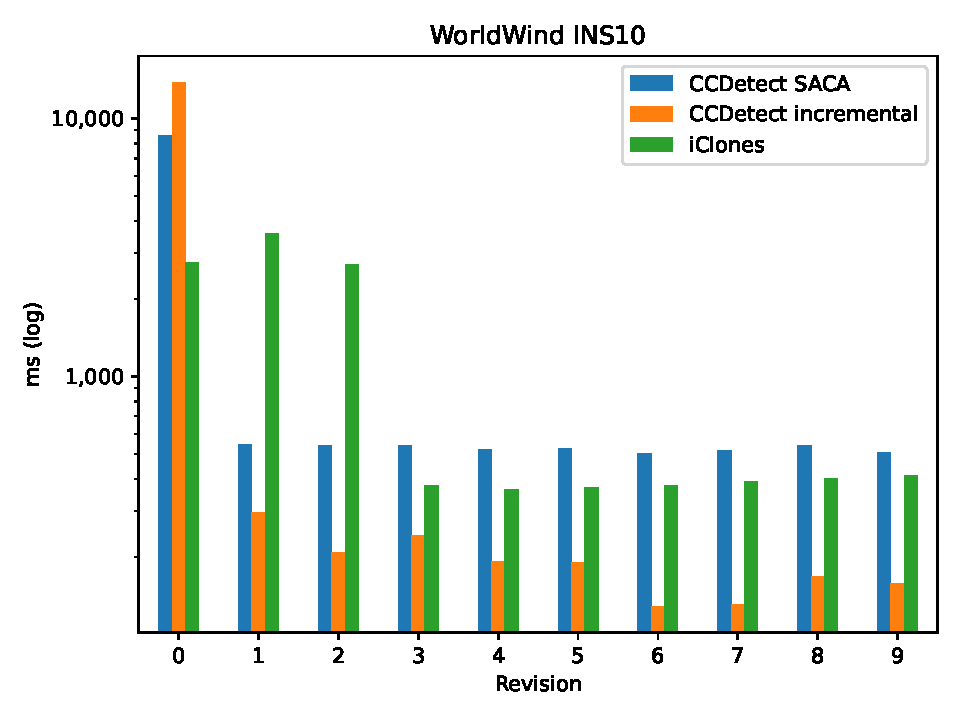
\includegraphics[width=0.49\textwidth]{figures/performancegraphs/WorldWind_INS10.pdf}
        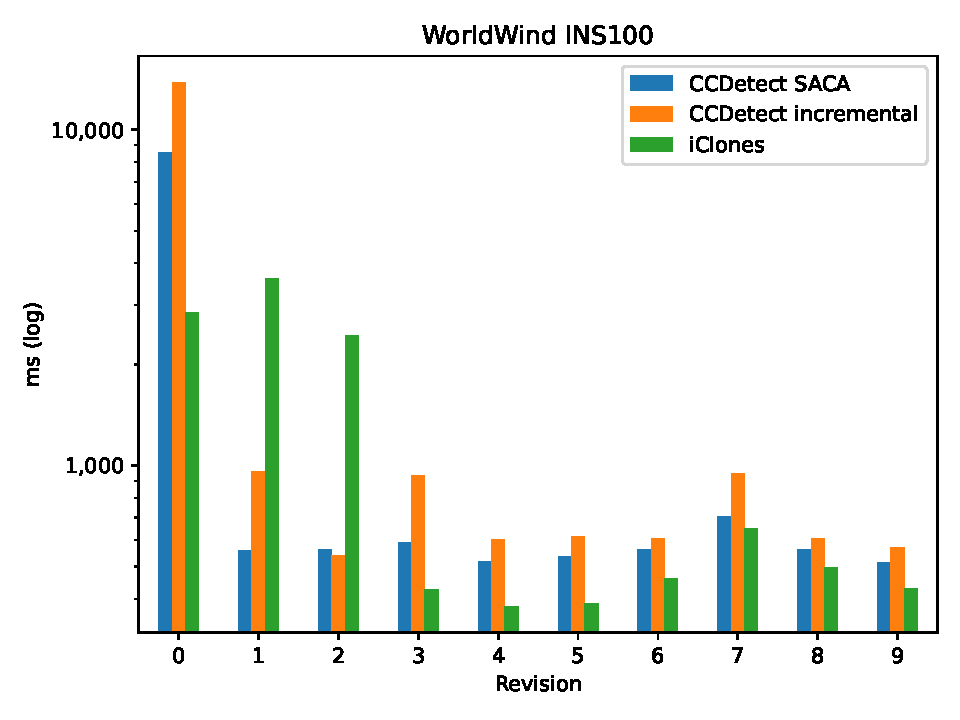
\includegraphics[width=0.49\textwidth]{figures/performancegraphs/WorldWind_INS100.pdf}
    \end{center}
    \caption{WorldWind performance benchmark}
    \label{fig:WorldWind}
\end{figure}

\end{frame}

\begin{frame}{neo4j (1MLOC)}
    \begin{figure}[H]
    \begin{center}
        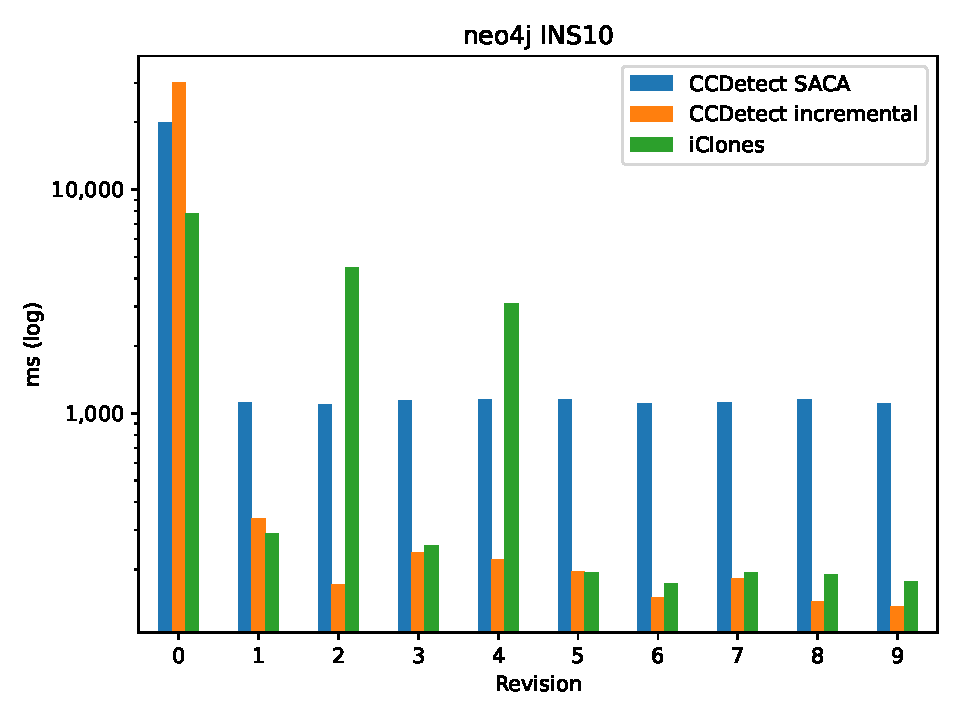
\includegraphics[width=0.49\textwidth]{figures/performancegraphs/neo4j_INS10.pdf}
        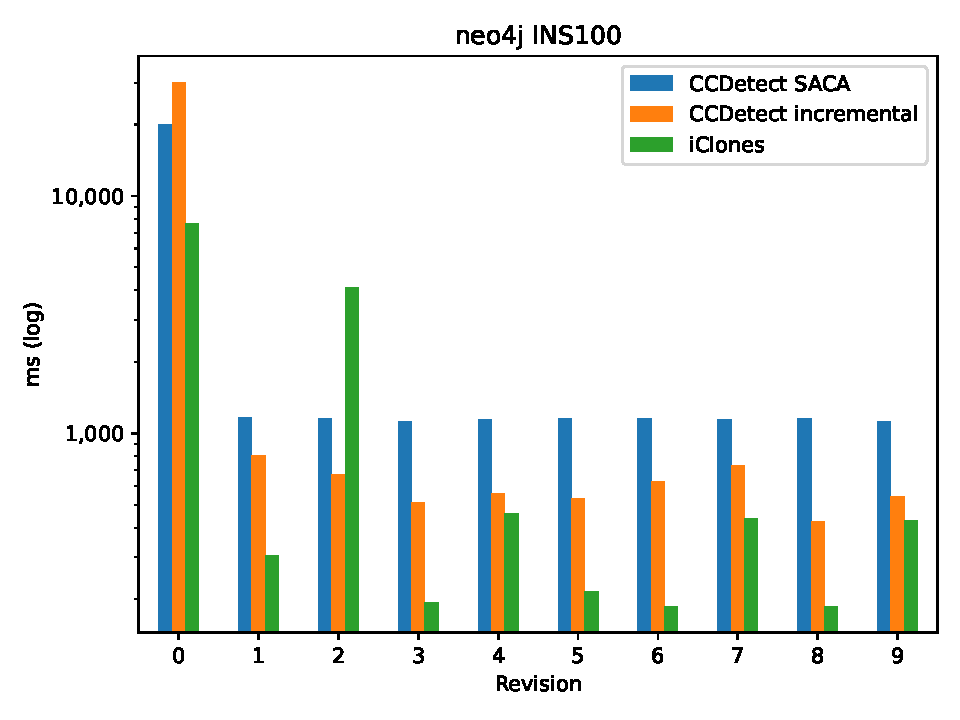
\includegraphics[width=0.49\textwidth]{figures/performancegraphs/neo4j_INS100.pdf}
    \end{center}
    \caption{neo4j performance benchmark}
    \label{fig:neo4j}
\end{figure}

\end{frame}

\begin{frame}{graal (2.2MLOC)}
    \begin{figure}[H]
    \begin{center}
        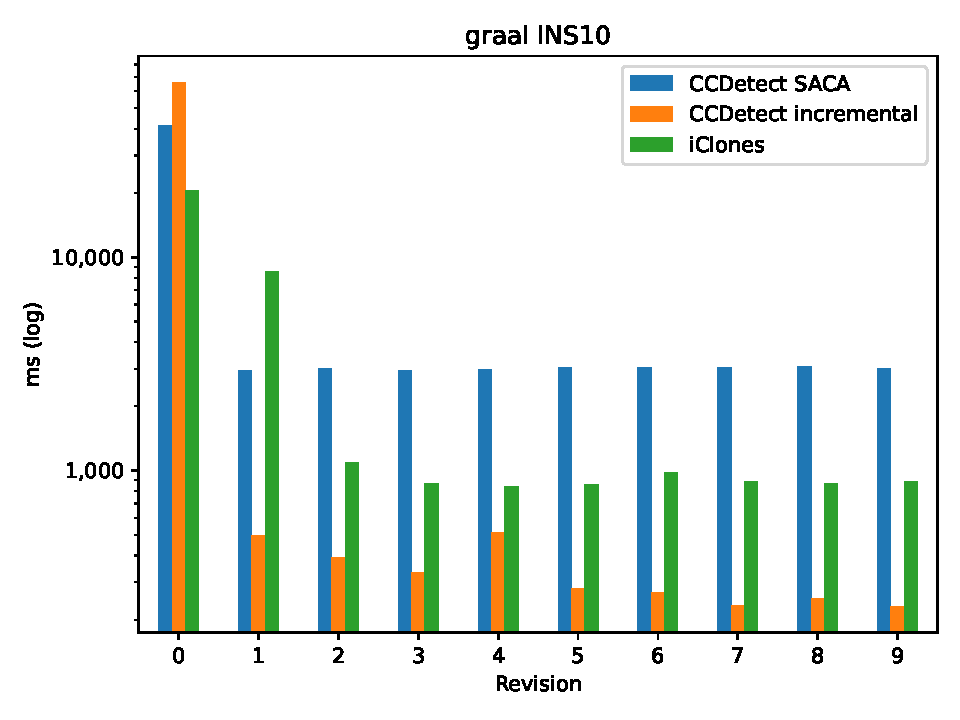
\includegraphics[width=0.49\textwidth]{figures/performancegraphs/graal_INS10.pdf}
        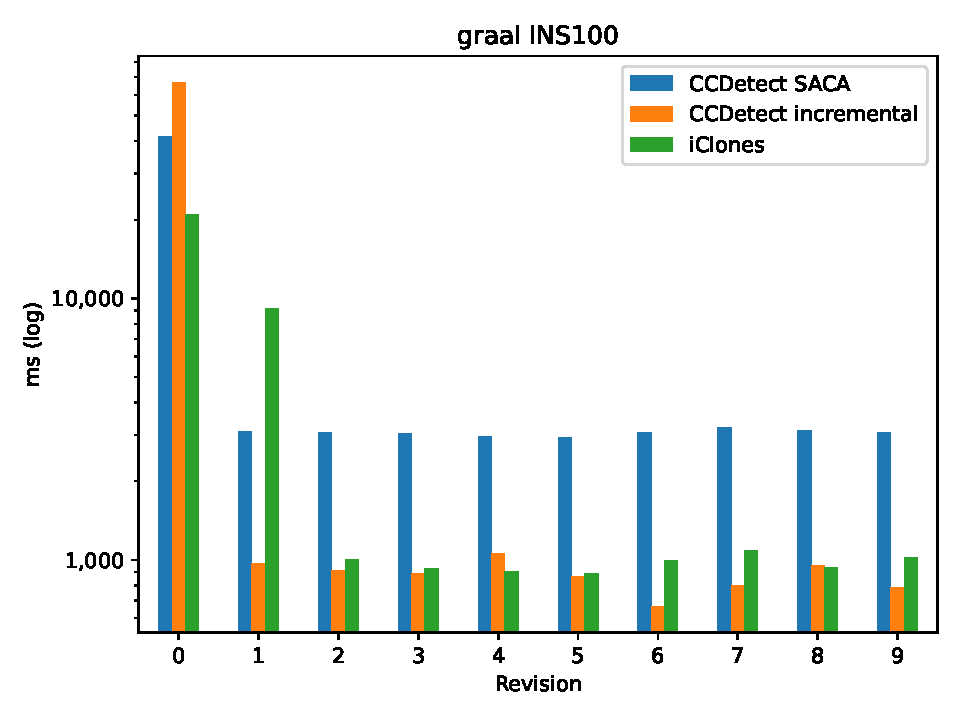
\includegraphics[width=0.49\textwidth]{figures/performancegraphs/graal_INS100.pdf}
    \end{center}
    \caption{graal performance benchmark}
    \label{fig:graal}
\end{figure}
\end{frame}

\begin{frame}{flink (2.3MLOC)}
    \begin{figure}[H]
    \begin{center}
        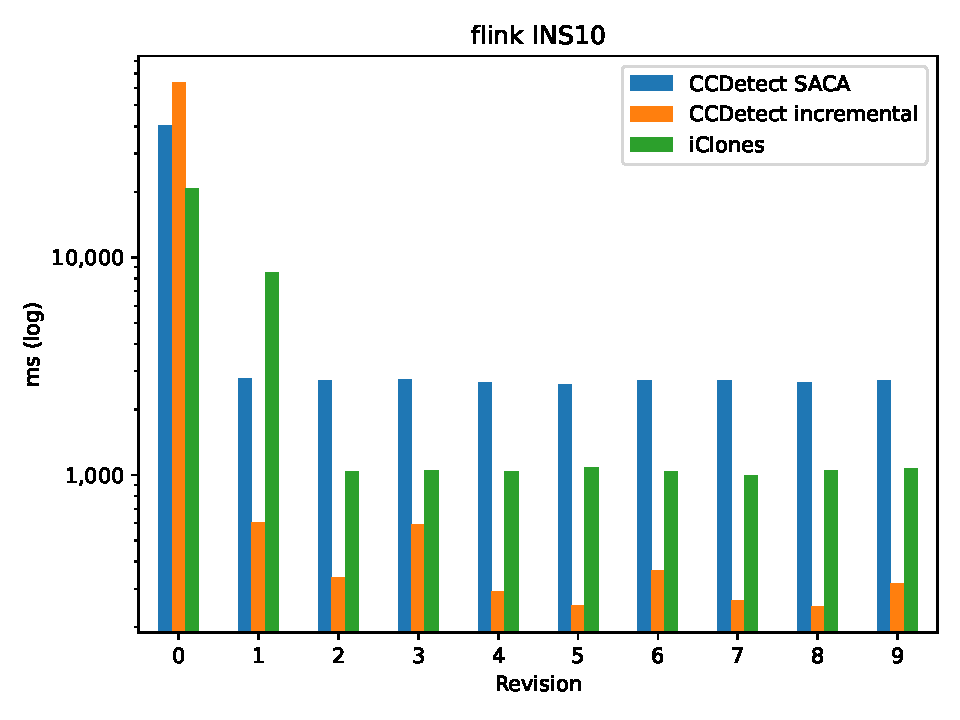
\includegraphics[width=0.49\textwidth]{figures/performancegraphs/flink_INS10.pdf}
        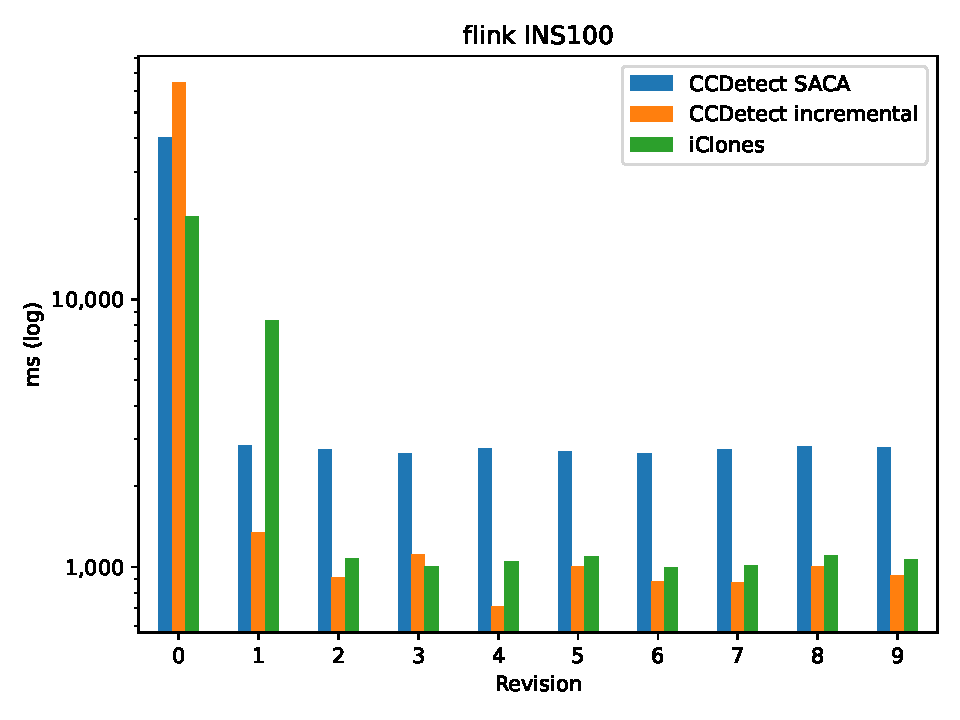
\includegraphics[width=0.49\textwidth]{figures/performancegraphs/flink_INS100.pdf}
    \end{center}
    \caption{flink performance benchmark}
    \label{fig:flink}
\end{figure}

\end{frame}

\begin{frame}{elasticsearch (3.2MLOC)}
    \begin{figure}[H]
    \begin{center}
        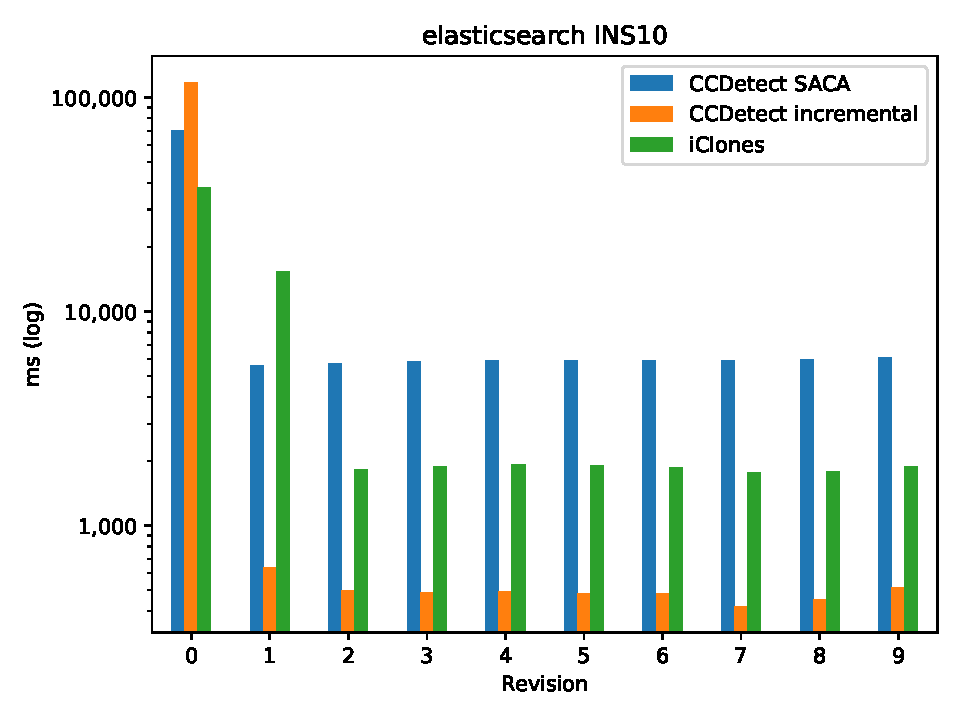
\includegraphics[width=0.49\textwidth]{figures/performancegraphs/elasticsearch_INS10.pdf} 
        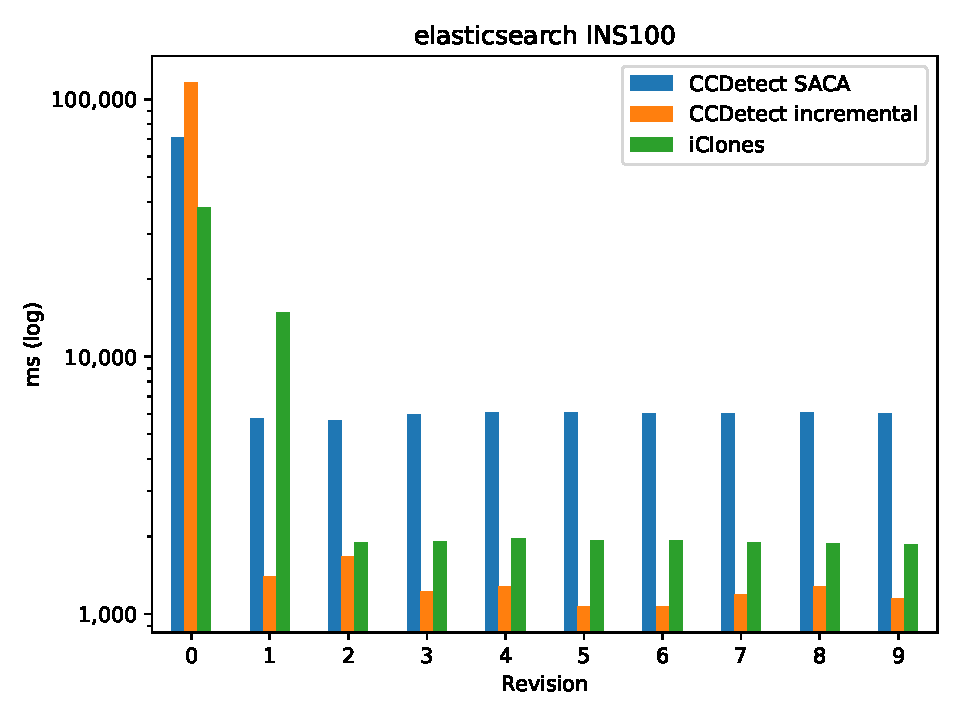
\includegraphics[width=0.49\textwidth]{figures/performancegraphs/elasticsearch_INS100.pdf} \end{center}
    \caption{elasticsearch performance benchmark}
    \label{fig:elasticsearch}
\end{figure}
\end{frame}

\begin{frame}{intellij-community (5.8MLOC)}
    \begin{figure}[H]
    \begin{center}
        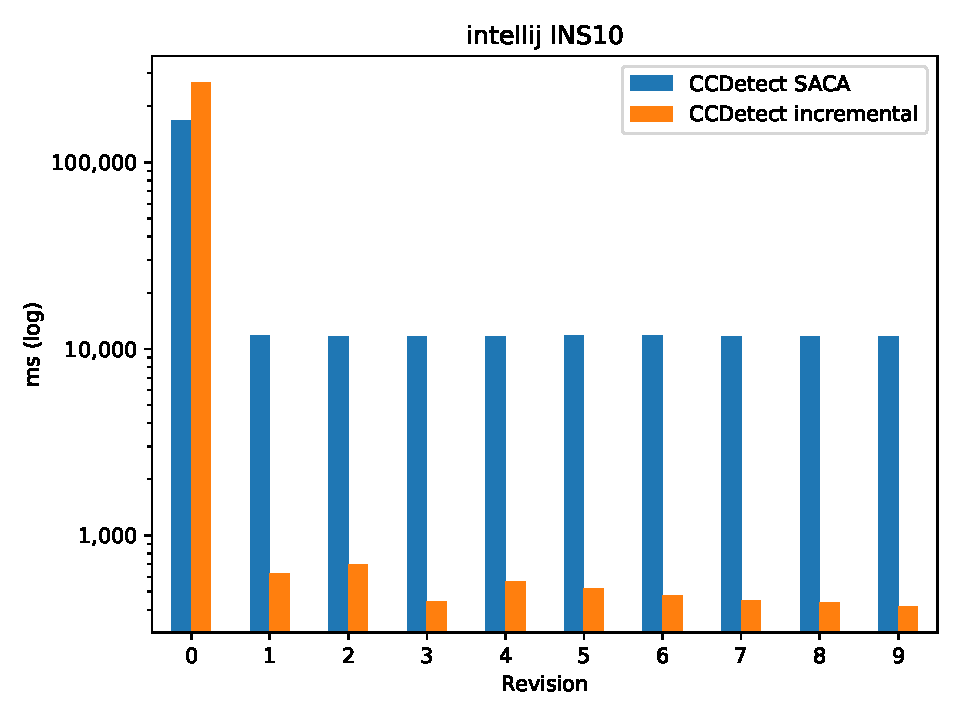
\includegraphics[width=0.49\textwidth]{figures/performancegraphs/intellij_INS10.pdf}
        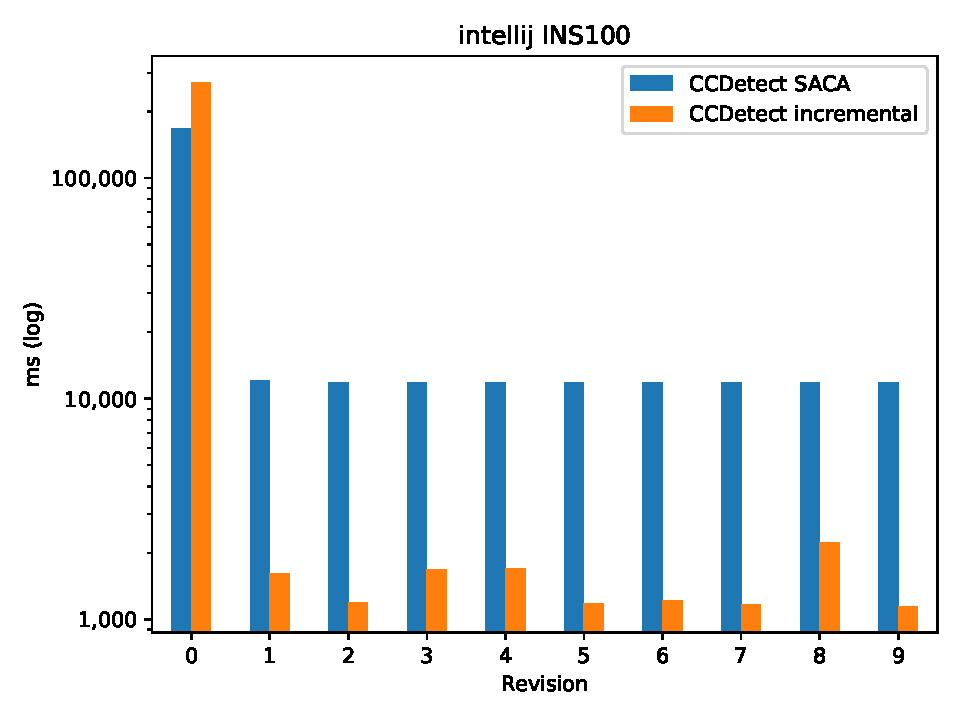
\includegraphics[width=0.49\textwidth]{figures/performancegraphs/intellij_INS100.pdf}
    \end{center}
    \caption{intellij-community performance benchmark}
    \label{fig:intellij}
\end{figure}
\end{frame}

\begin{frame}{elasticsearch (3.2MLOC)}
    \begin{figure}[H]
    \begin{center}
        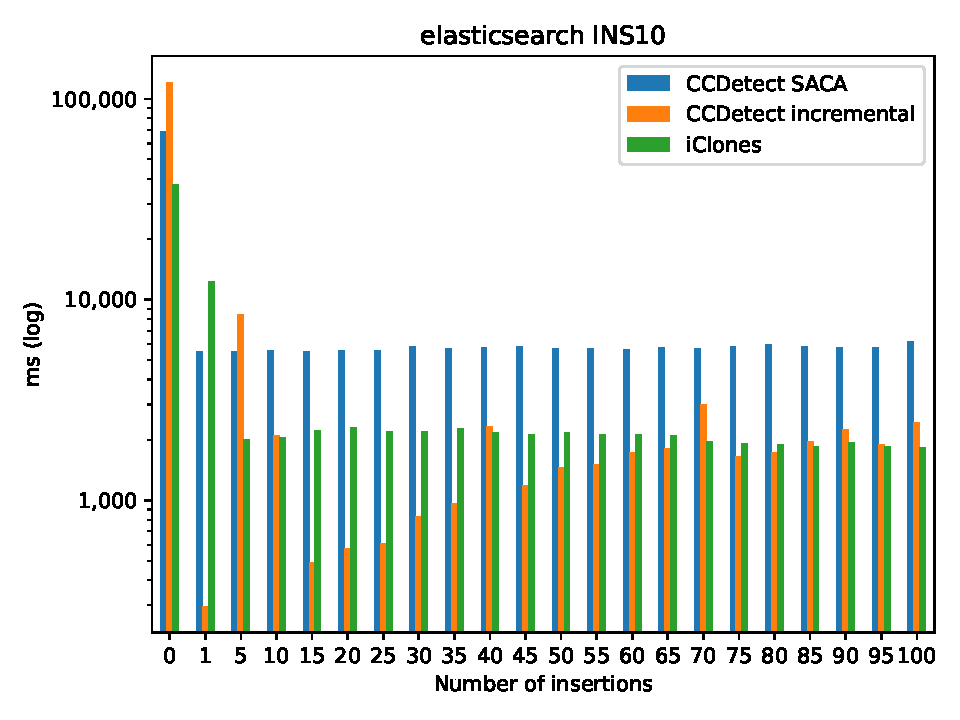
\includegraphics[width=0.49\textwidth]{figures/incedit_performancegraphs/elasticsearch_INS10.pdf}
        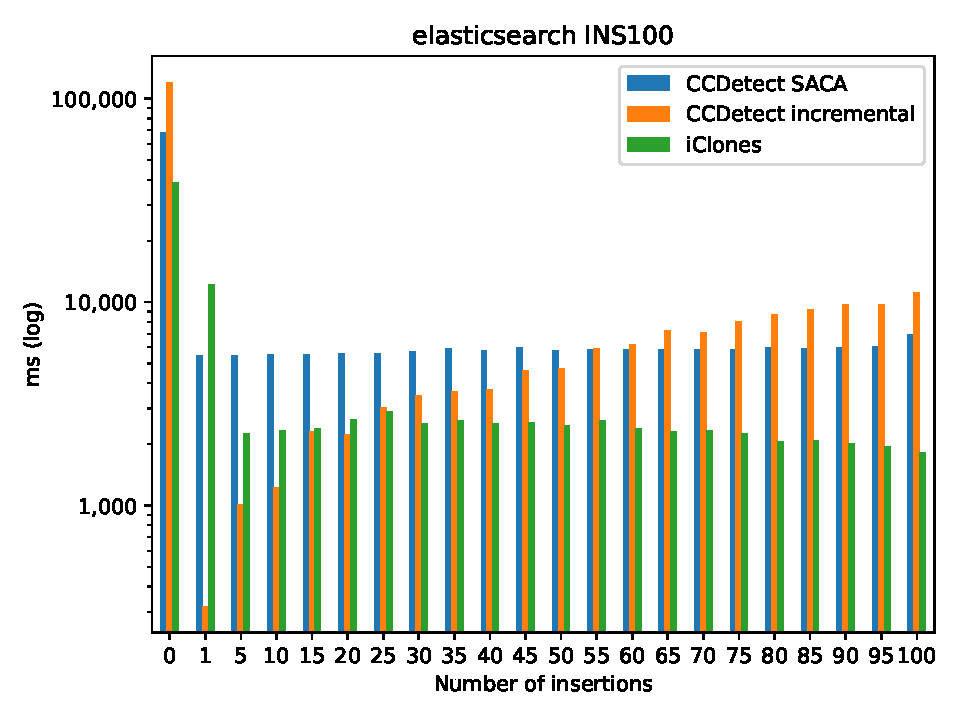
\includegraphics[width=0.49\textwidth]{figures/incedit_performancegraphs/elasticsearch_INS100.pdf}
    \end{center}
    \caption{Elasticsearch performance benchmark with increasing number of edits}
    \label{fig:elasticsearch_inc}
    \end{figure}
\end{frame}

\begin{frame}{Memory usage}
    \begin{figure}[H]
    \begin{center}
        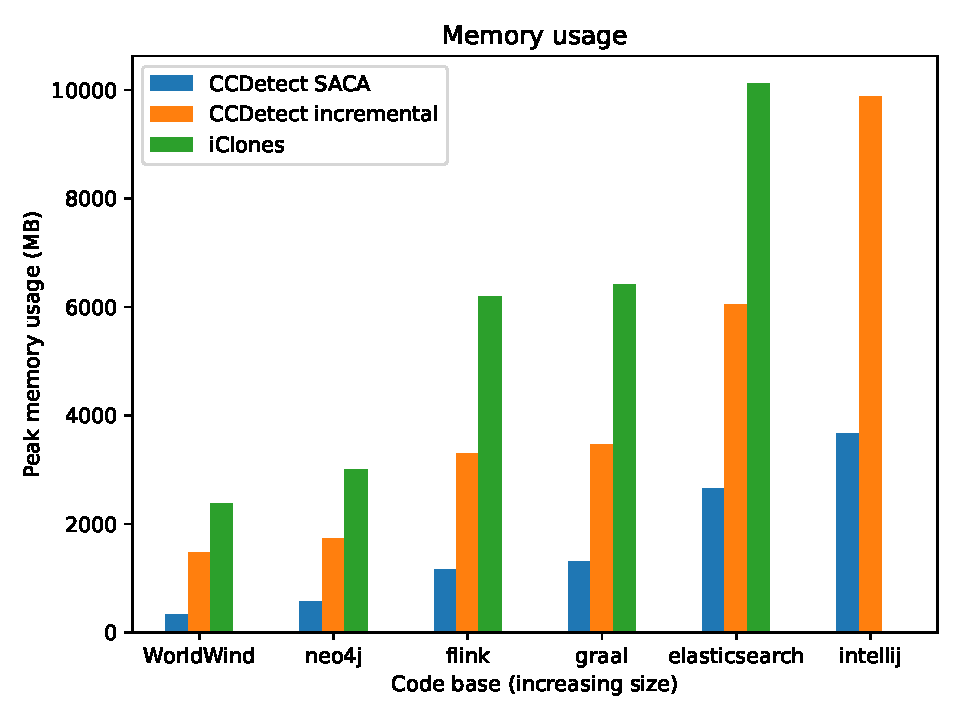
\includegraphics[width=0.6\textwidth]{figures/memoryusage.pdf}
    \end{center}
    \caption{Peak memory usage of each tool when running the DEL10 test for each code base.}
    \label{fig:memoryusage}
\end{figure}
\end{frame}

\begin{frame}{Language and IDE agnostic}
    \begin{itemize}
        \item CCDetect-LSP tested on 6 languages
            \begin{itemize}
                \item Java
                \item Python
                \item C
                \item Rust
                \item Javascript
                \item Go
            \end{itemize}
        \item And 2 IDEs
            \begin{itemize}
                \item Neovim
                \item VSCode
            \end{itemize}
        \item Works well in our experience
    \end{itemize}

\end{frame}
    
\section{Discussion}
\begin{frame}{Discussion}
    \begin{itemize}
        \item Performance and memory usage
            \begin{itemize}
                \item Incremental detection has the best performance if edits are ``small''
                \item Memory usage is lower than other incremental algorithms, but could still be a
                    bottle-neck for practical use
            \end{itemize}
        \item Language- and IDE agnostic
            \begin{itemize}
                \item Works well for any language if grammar is correct
                \item Setup and configuration depends on the IDE
            \end{itemize}
		\item Practical usage in the IDE scenario
            \begin{itemize}
                \item Live manual/automatic refactoring of code clones
                \item Clone information used by other tools/refactorings
            \end{itemize}
    \end{itemize}
\end{frame}

\section{Conclusion}
\begin{frame}{Conclusion}
	\begin{itemize}
        \item CCDetect-LSP is a performant incremental clone detection tool
            \begin{itemize}
                \item Facilitates fast incremental updates
                \item Lower memory usage than existing solutions
                \item Language- and IDE agnostic clone detection
            \end{itemize}
		\item Future work
            \begin{itemize}
                \item Type-3 clones
                \item Refactoring clones
                \item Compressing data structures
            \end{itemize}
	\end{itemize}
\end{frame}

\section{Questions or demo?}

\begin{frame}{LSP}
    \begin{figure}
        \begin{center}
            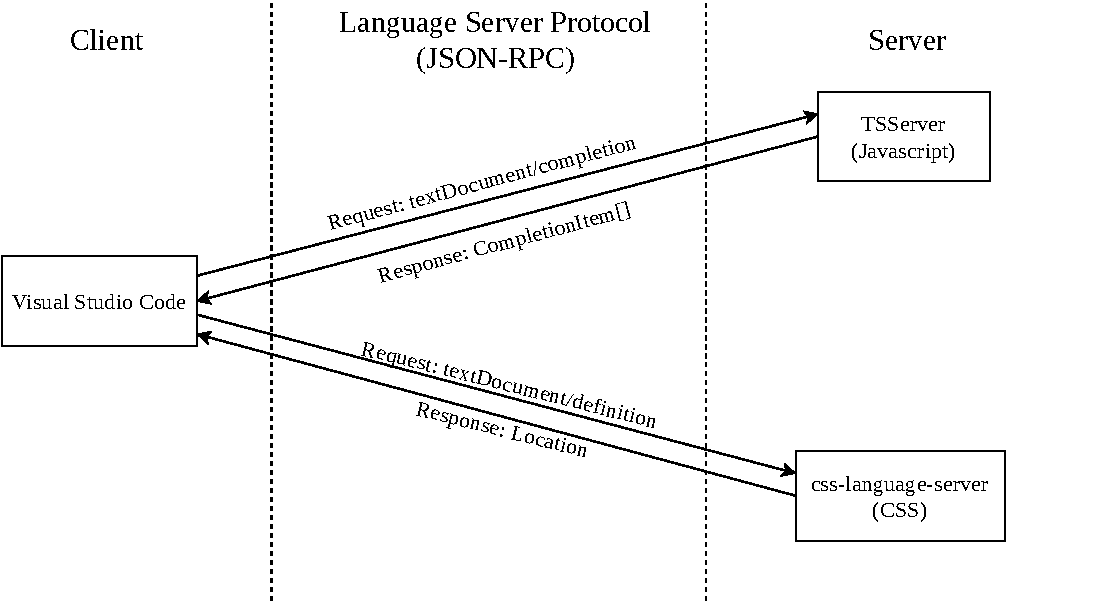
\includegraphics[width=0.7\textwidth]{figures/lspcommunication.drawio.pdf}
        \end{center}
        \caption{Example LSP server communication}
    \end{figure}
\end{frame}

\begin{frame}{LSP architecture}
    \begin{figure}
        \begin{center}
            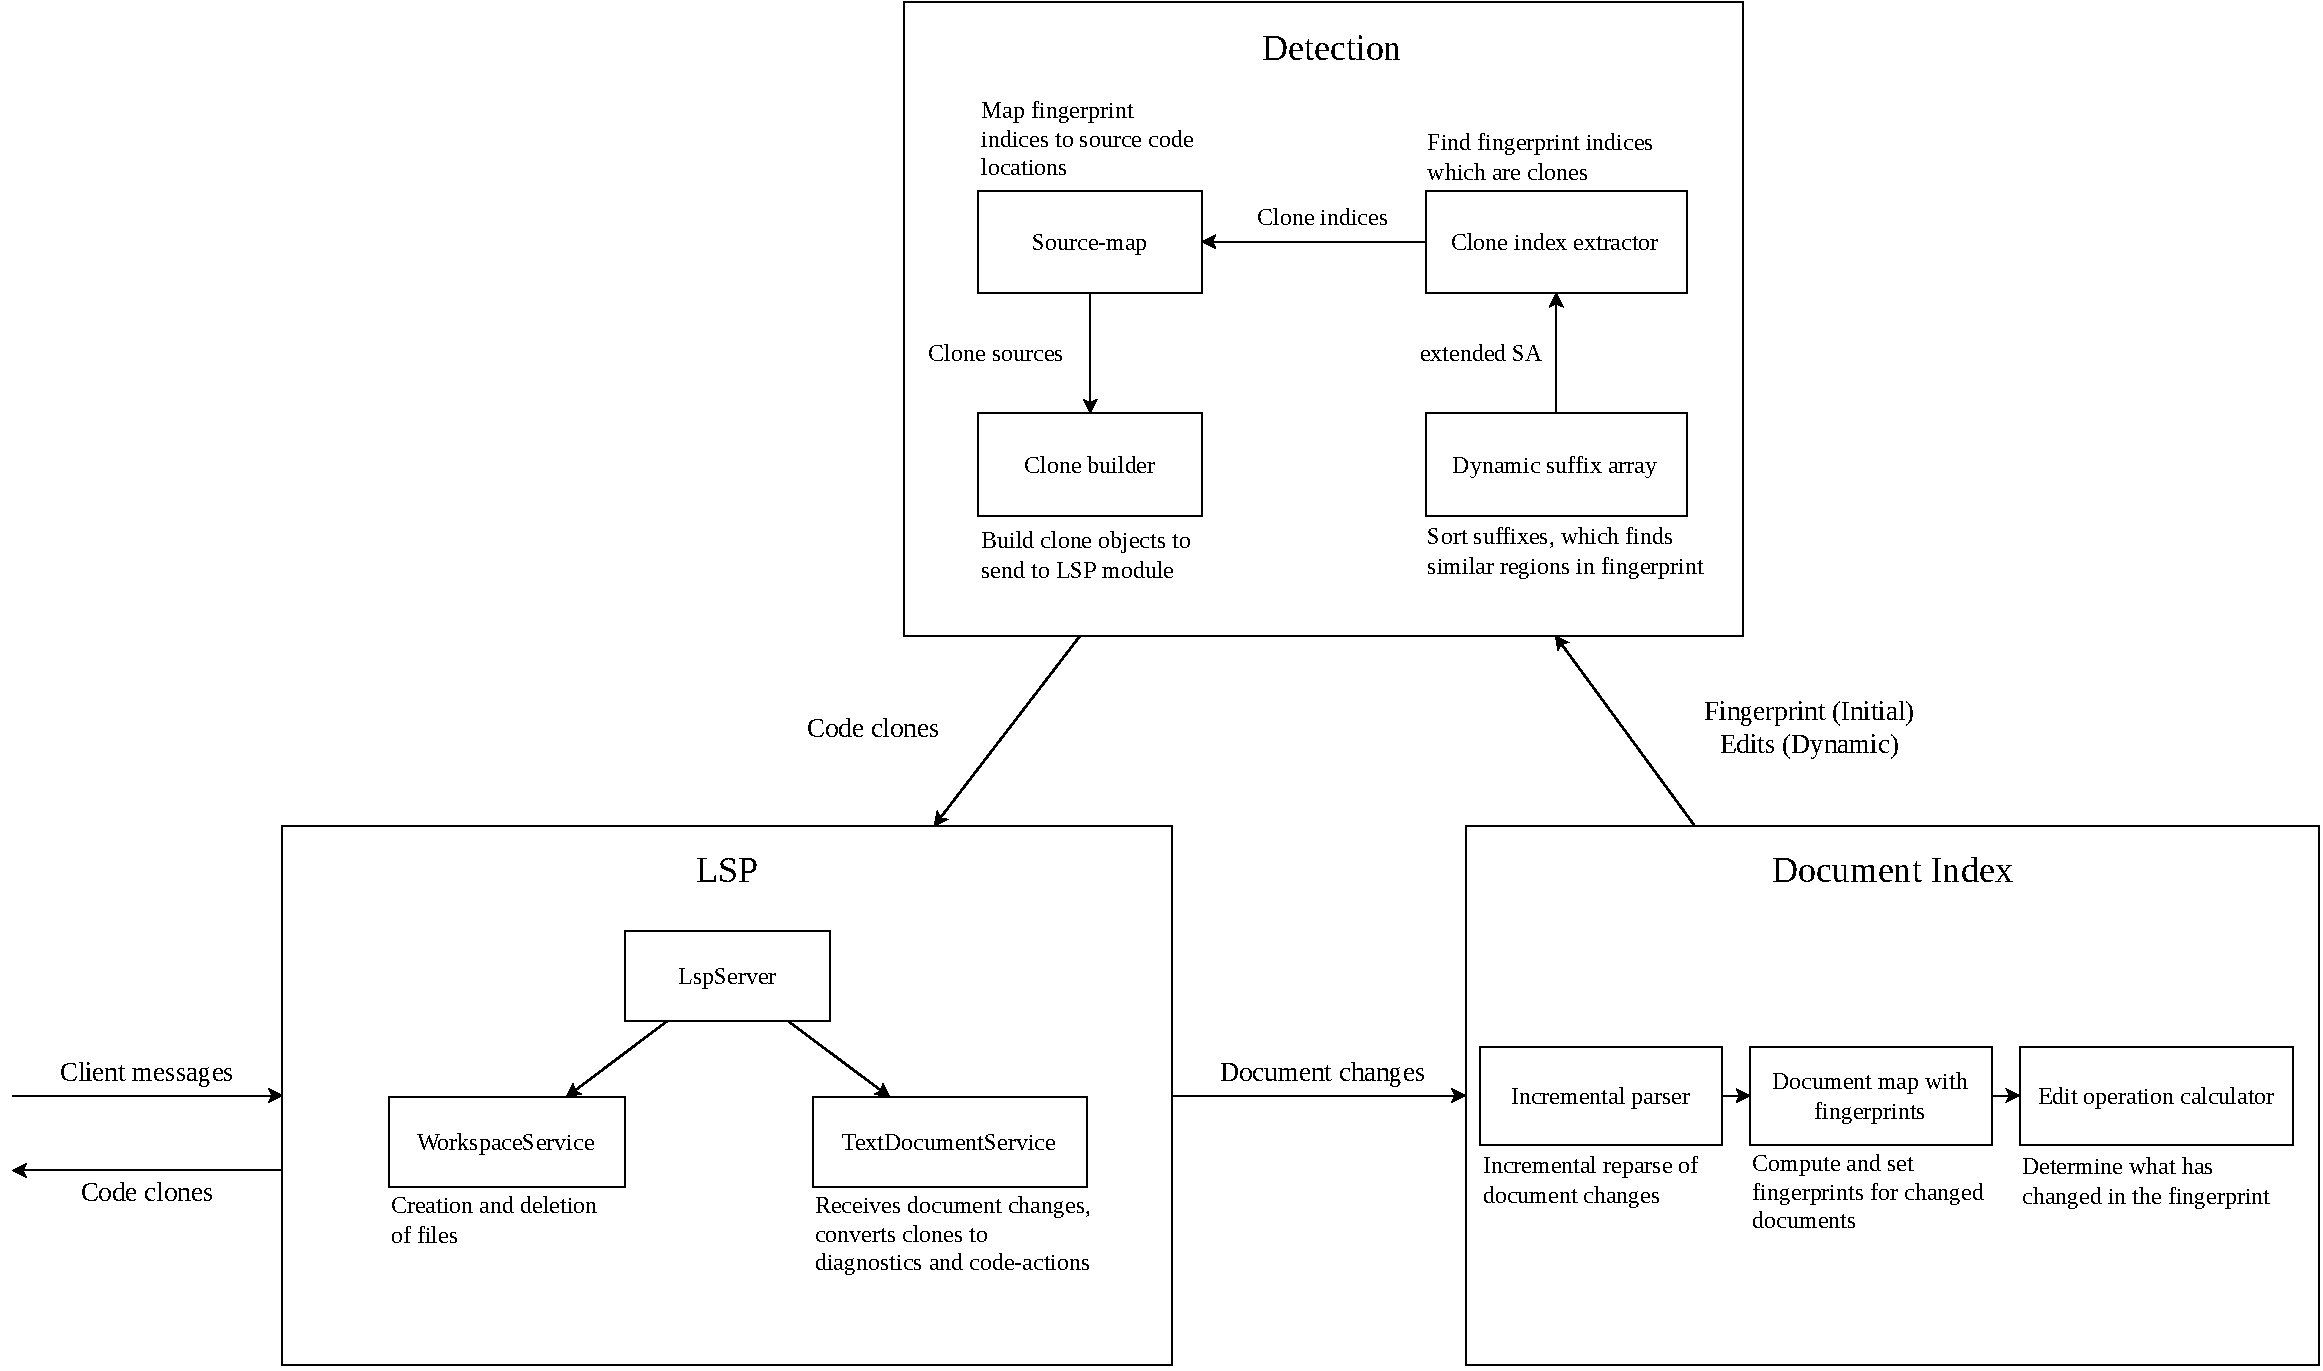
\includegraphics[width=0.7\textwidth]{figures/architecture.drawio.pdf}
        \end{center}
        \caption{Architecture of CCDetect-LSP}
    \end{figure}
\end{frame}

\begin{frame}[fragile]
	\frametitle{Clone types: type-3 and type-4}
    \vspace{0.5cm}
	\begin{figure}[t]
		\begin{center}
			\begin{tabular}{p{6cm} | p{6cm}}
				\begin{lstlisting}
for (int i = 0; i < 10; i++) {
    print(i);
}\end{lstlisting} &
				\begin{lstlisting}
for (int i = 0; i < 10; i++) {
    print(i);
    print(i*2);
}\end{lstlisting}
			\end{tabular}
		\end{center}
		\caption{Type-3 clone pair}
		\label{fig:type3clone}
	\end{figure}
    \vspace{-0.5cm}

	\begin{figure}[t]
		\begin{center}
			\begin{tabular}{r | p{6.5cm}}
				\hspace{3.2cm}\begin{lstlisting}
print((n*(n-1))/2)
\end{lstlisting} &
				\begin{lstlisting}
int sum = 0;
for (int i = 0; i < n; i++) {
    for (int j = i+1; j < n; j++) {
        sum++;
    }
}
print(sum);
            \end{lstlisting}
			\end{tabular}
		\end{center}
		\caption{Type-4 clone pair}
		\label{fig:type4clone}
	\end{figure}
\end{frame}

\end{document}

